\documentclass[tikz,border=10pt]{standalone}
\usepackage{amsmath}
\usetikzlibrary{arrows.meta, positioning, calc, decorations.pathreplacing}

\definecolor{c1}{HTML}{000000}
\definecolor{c2}{HTML}{233D4D}
\definecolor{c3}{HTML}{FE7F2D}
\definecolor{c4}{HTML}{EAECF0}
\definecolor{axiscolor}{HTML}{333333}
\definecolor{labelcolor}{HTML}{5F6B75}

\begin{document}
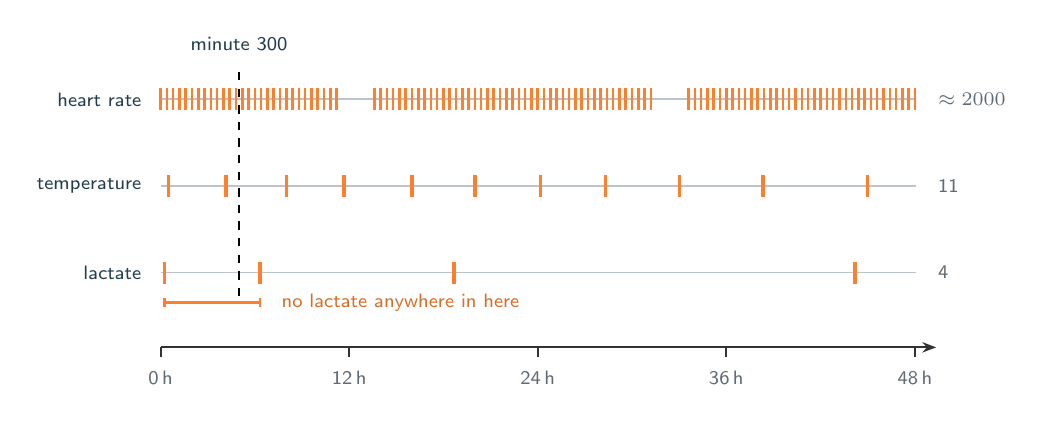
\begin{tikzpicture}[
    every node/.style={font=\sffamily},
    lab/.style={font=\sffamily\scriptsize, text=labelcolor},
    tag/.style={font=\sffamily\scriptsize, text=c2},
    hot/.style={font=\sffamily\scriptsize, text=c3!85!black},
]

% minute m  ->  x = 1.20 + m*0.003333
\def\X#1{1.20 + #1*0.003333}

% ---------------------------------------------------------------- lanes
\foreach \y/\name in {5.60/heart rate, 4.50/temperature, 3.40/lactate}{
    \node[tag, anchor=east] at (1.08, \y) {\name};
    \draw[c2!30, line width=0.6pt] (1.20, \y) -- (10.80, \y);
}

% heart rate: a reading most minutes, with two dropouts
\foreach \m in {0,24,...,2880}{
    \pgfmathparse{((\m>690)&&(\m<810)) || ((\m>1890)&&(\m<2010)) ? 0 : 1}
    \ifnum\pgfmathresult=1
        \draw[c3, line width=0.9pt] ({\X{\m}}, 5.46) -- ({\X{\m}}, 5.74);
    \fi
}
\node[lab, anchor=west] at (10.95, 5.60) {$\approx 2000$};

% temperature: eleven times
\foreach \m in {30, 250, 480, 700, 960, 1200, 1450, 1700, 1980, 2300, 2700}{
    \draw[c3, line width=1.2pt] ({\X{\m}}, 4.36) -- ({\X{\m}}, 4.64);
}
\node[lab, anchor=west] at (10.95, 4.50) {11};

% lactate: four
\foreach \m in {15, 380, 1120, 2650}{
    \draw[c3, line width=1.4pt] ({\X{\m}}, 3.26) -- ({\X{\m}}, 3.54);
}
\node[lab, anchor=west] at (10.95, 3.40) {4};

% ---------------------------------------------------------------- minute 300
\draw[c1, line width=0.8pt, dashed] ({\X{300}}, 3.10) -- ({\X{300}}, 6.05);
\node[tag, anchor=south] at ({\X{300}}, 6.10) {minute 300};
\node[hot] at ({\X{300}}, 3.05) {};
\draw[c3, line width=1.0pt] ({\X{15}}, 3.02) -- ({\X{380}}, 3.02);
\draw[c3, line width=1.0pt] ({\X{15}}, 2.96) -- ({\X{15}}, 3.08);
\draw[c3, line width=1.0pt] ({\X{380}}, 2.96) -- ({\X{380}}, 3.08);
\node[hot, anchor=west] at ({\X{380}+0.15}, 3.02)
    {no lactate anywhere in here};

% ---------------------------------------------------------------- axis
\draw[axiscolor, line width=0.8pt, -{Stealth[length=5pt]}]
    (1.20, 2.45) -- (11.05, 2.45);
\foreach \h in {0, 12, 24, 36, 48}{
    \pgfmathsetmacro\m{\h*60}
    \draw[axiscolor, line width=0.7pt] ({\X{\m}}, 2.45) -- ({\X{\m}}, 2.33);
    \node[lab, anchor=north] at ({\X{\m}}, 2.27) {\h\,h};
}

\end{tikzpicture}
\end{document}
